\chapter{Alternating Current and Time Varying Signals}

\section{Introduction}
In this lab you will use two essential new pieces of lab equipment
(scope and function generator) to study alternating current and time
varying signals.

\section{Function Generator}

\begin{figure}[htbp]
\begin{center}
\begin{circuitikz}[line width=1pt]
\draw (0,0) to[sinusoidal voltage source,bipoles/length=1.5cm] ++(0,3.0) to[short] ++(2.0,0) coordinate(X) to[short,*-o] ++(1.0,0) node[right]{A};
\draw (X) to[R,-*] ++(0,-3.0) coordinate(X) to[short,-o] ++(1.0,0) node[right]{B};
\draw (X) to[short,-*] ++(-2.0,0) node[ground,yscale=2.0]{};
\end{circuitikz} 
\caption{A function generator driving a resistor.}
\label{fig:mycirc}
\end{center}
\end{figure}

Connect the output of Channel 1 directly to the Voltage measurement
input of your Triplett 9007 DMM, using a BNC to banana plug adapter as
shown in Fig.~\ref{}.  Set your DMM to the 20 V AC scale (the V with a
squiggly line) .

Now set your function generator to the factory default: 
\begin{displaymath}
\rm Utility\;Button \to System \to Set\;to\;Default \to Select.
\end{displaymath}
You must perform this step today for the instructions that follow to make sense.  With shared equipment, it is essential to know how to restore the factory default, in case another user has left the device with strange settings.  You don't need to start with this step every lab, but it is a fast way to recover when you encounter strange behavior.

The factory default settings place the function generator in Sine function mode, so leave that set as is.

Adjust the frequency to $10~\rm kHz$ by turning the large knob.  Press the Freq/Period choice button twice to see how you can switch between specifying frequency and period.  Leave it as Frequency for now.

You can likewise switch between Ampl and Offset to specify an amplitude and an offset, or set the high and low values.  Adjust the amplitude to $1~{\rm V}$ RMS by:
\begin{displaymath}
\rm Ampl \to 1 \to Vrms
\end{displaymath}

Your function generator should now be set to provide a $10~\rm kHz$ Sine function with an RMS amplitude of $1~\rm V$.  Confirm this from the status screen.

Note that your DMM reads $0~\rm V$.  Because the output is not yet enabled!  Press the "On/Off" button above Channel 1 to enable the output.

%Now your DMM reads something non-zero... but quite a bit different from the $1 V$ RMS we expect.  What gives?  Your DMM\footnote{https://triplett.com/product/digital-multimeter-model-9007-a/} is only rated to $2~\rm kHz$!  

Turn the output frequency of your function generator down to $2~\rm kHz$.  Now your DMM should read an RMS voltage near $2~\rm V$, about twice the value that we expect.  (EXPLAIN)

\begin{figure}[htbp]
\begin{center}
\begin{tabular}{cc}
\begin{circuitikz}[line width=1pt]
\draw (0,0) to[sinusoidal voltage source,bipoles/length=1.25cm] ++(0,1.5) to[R,l_=$R_{\rm S}$] ++(0,1.5) to[short] ++(2.0,0) coordinate(X) to[short,*-o] ++(1.0,0) node[right]{A};
\draw (X) to[R,-*,l=$R_{\rm L}$] ++(0,-3.0) coordinate(X) to[short,-o] ++(1.0,0) node[right]{B};
\draw (X) to[short,-*] ++(-2.0,0) node[ground,yscale=2.0]{};
\end{circuitikz} & 
\begin{circuitikz}[line width=1pt]
\draw (0,0) to[sinusoidal voltage source,bipoles/length=1.25cm] ++(0,1.5) to[R,l_=$R_{\rm S}$] ++(0,1.5) to[short,-o] ++(2.0,0) coordinate(X) node[right]{A};
\draw (0,0) node[ground,yscale=2.0]{} to[short,-o] ++(2.0,0) node[right]{B};
\end{circuitikz} \\
(a) & (b) \\
\end{tabular}
\caption{A function generator with source impedance explicitly shown.}
\label{fig:funcimpedance}
\end{center}
\end{figure}

(Adjust DC offset and measure DC voltage with DMM)

%Connect the output of your function generator as input to your volt meter using a coaxial cable and banana plug adapter, as shown in Fig.~X.
%Set your function generator to an output impedance of $50~\Omega$ by...
%Set the function generator to produce a 1 kHz sine wave with an RMS voltage of 1.0 V.
%Now measure the AC voltage using your voltmeter.  Record the value reported by your voltmeter.

%Now set the output impedance to high impedance, set the output to $1.0~\rm V$, and repeat the measurement.  What's going on here?

%Your function generator has an output impedance of $50~\Omega$ which ensures that you cannot short circuit it.  However, when driving $50~\Omega$ loads...

\section{Oscilloscope}

Trigger...

AC coupled versus DC bias...

Grounding???


To observe the time dependence of signals, the tool of choice is the oscilloscope.

Press the default setup function of yours scope...

Adjust the trigger level and observe that the phase of the channel 1...

\section{Lissajous Figures}

Lissajous figures are the graph of system of two parameterized functions:
\begin{eqnarray*}
x &=& A_1 \sin(2 \pi f_1 t + \delta) \\
y &=& A_2 \sin(2 \pi f_2 t) 
\end{eqnarray*}
which produces a closed loop if the ratio $A_1 / A_2$ is rational.  The appearance of the figure is of a 3 dimensional knot with the viewing angle determined by the parameter $\delta$.  Two examples are shown in Fig.~\ref{fig:tracelissajous}.

To begin, adjust channel 2 of your scope as you did channel 1: probe to 1x, with $500~mV$ range.
Connect the output of Channel 2 on your function generator to the channel 2 input on your ...
Set the amplitude of both Channel 1 and Channel 2 to $3~\rm V$ peak-to-peak.

The relative phase between the two output channels of your function generator shifts whenever you adjust the frequency of one of the signals.  For consistent results with offline plots and the scope traces shown here, you'll need to align the phase of the two channels every time you adjust the frequency:
\begin{displaymath}
\rm Inter Ch button \to AlignPhase.
\end{displaymath}
You should now have reproduced the "start" pattern from Fig.~\ref{fig:tracelissajous}a.

Adjust the phase of Channel 2 until the pattern collapses into a Fish pattern (or greek letter $\alpha$).
Save a scope trace by inserting your USB drive into the scope and pressing the Save button.  Then produce the parabola and lace patterns, according to the settings in the table, saving a scope trace each time.  Remember to align the phase each time you change the frequency.

Next, produce the crown pattern, shown in Fig.~\ref{fig:Lissajous}b.   For the right proportions, you'll need to adjust the amplitude of Channel 2 to $1~\rm V$ peak-to-peak, leaving Channel 1 at $3~\rm V$ peak-to-peak.  Notice that as you adjust the phase of Channel 1, the crown appears to rotate.  Adjust the frequency of Channel 2 to $4.0002~\rm kHz$.  The crown should now appear to rotate constantly at low speed.   This is a {\bf sign off} point in the lab.

\section{Analysis}

From the previous section, you should have scope traces for the fish, parabola, and crown.  Reproduce each of these figures using scientific python to draw the parameterized shape.  For example. Fig.~\ref{fig:pythonlissajous}.

One way to approach this problem is to set the period to $1~\mu s$, with fundamental angular frequency $\omega = 2 \pi~\rm kHz$.  

One way to approach this problem is to set the period to $1~\mu s$.  The functions should be evaluated at 1000 discrete times within the interval from 0 to $1~\mu s$.
\begin{verbatim}
     t = np.linspace(0,1,num=1000)
\end{verbatim}
Define a fundamental angular frequency $\omega_0 = 2 \pi~\rm kHz$:
\begin{verbatim}
     w = 2*np.pi~\rm kHz
\end{verbatim}
With these definitions, we would define:
\begin{verbatim}
     x = np.sin(4*w*t)
\end{verbatim}
to obtain $x$ points corresponding to $f=4~\rm kHz$ sine function.

When plotting your curves, use:
\begin{verbatim}
       plt.axis('equal')
\end{verbatim}
to keep the unit aspect ratio used by your scope.

\begin{figure}[htbp]
\begin{center}
\begin{tabular}{cc}
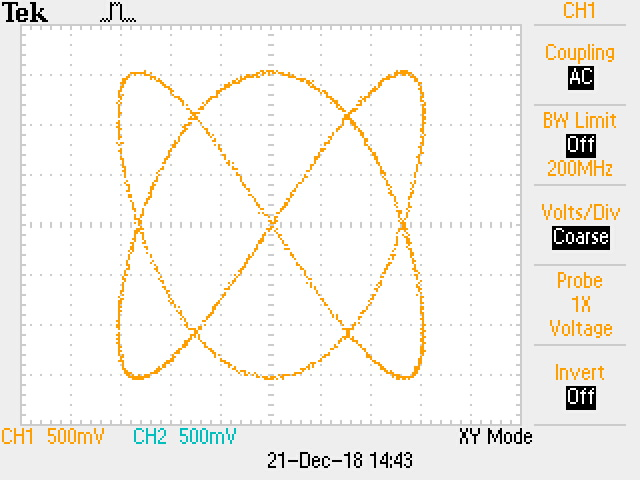
\includegraphics[width=0.45\textwidth]{figs/labs/lissajous/scope_lissajous.jpg} & 
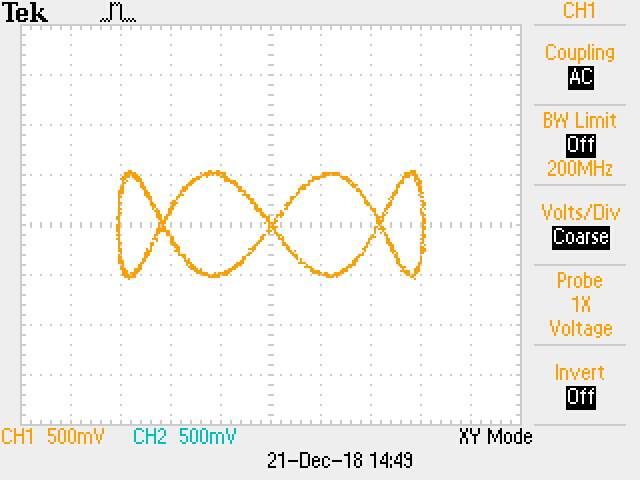
\includegraphics[width=0.45\textwidth]{figs/labs/lissajous/scope_crown.jpg} \\
(a) & (b) \\
\end{tabular}
\caption{Scope traces from Lissajous figures from settings for (a) start, and (b) crown.}
\label{fig:tracelissajous}
\end{center}
\end{figure}

\begin{table}
\caption{Settings for various Lissajous figures.}
\begin{tabular}{llll}
pattern & $f_1~\rm(kHz)$ & $f_2~\rm(kHz)$ & $\delta_1$ \\
start & 2 & 3 & 0 \\
fish & 2 & 3 & $30^\circ$ \\
parabola & 1 & 2 & $45^\circ$ \\
lace & 13 & 12 & 0 \\
crown & $1~\rm kHz$ & $4~\rm kHz$ & 0 \\
\end{tabular}
\end{table}

\begin{figure}[htbp]
\begin{center}
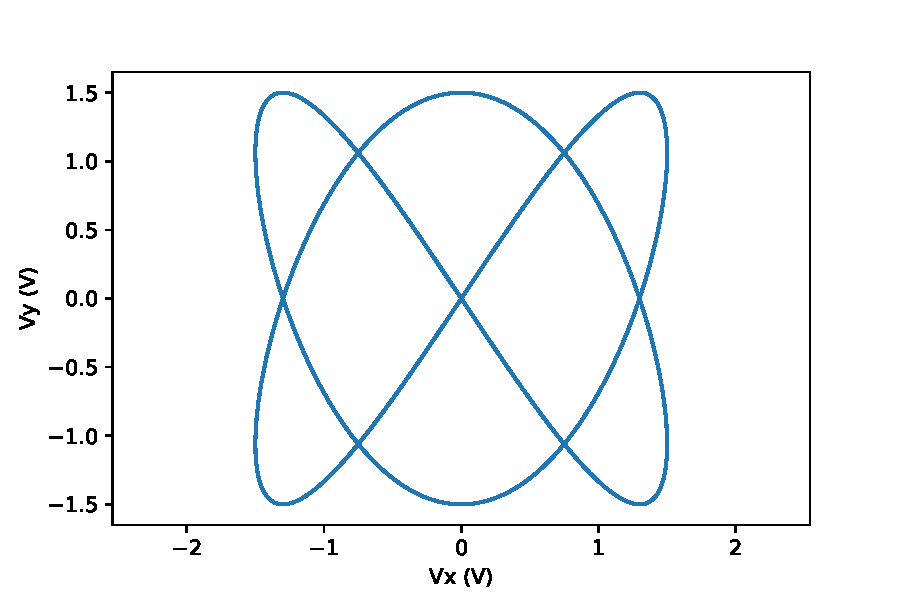
\includegraphics[width=0.45\textwidth]{figs/labs/lissajous/pythonlissajous.pdf} 
\caption{Lissajous curve constructed using Scientific Python corresponding to the scope trace in Fig.~\ref{fig:tracelissajous}a.}
\label{fig:pythonlissajous}
\end{center}
\end{figure}


figs/labs/lissajous/pythonlissajous.pdf

